\section{第一类:扫描时进行阴影计算}
Appel\cite{2}\cite{3}和之后的Bouknight, Kelley\cite{5}展示了渲染阴影的方法:在扫描图片的时候计算阴影边界。
Appel通过扩展他对于量化不可见性的概念来探测阴影边界。
量化不可见性是一种对于隐藏一个顶点的表面数量的度量。(假设是多边形物体)
这样的话,仅当一条线段上的所有点都是值为零的量化不可见性时,这条线段才是可见的。
Appel的隐藏表面算法可以探测到线段上量化不可见性的变化,然后只画出可见的部分。
这种方法产生一条线段绘制。\\
在扫描时决定阴影表面,同样也可以用来遮盖线段绘制。
通过在相等空间的水平线上和图片平面相交,产生穿过出射点的“切”平面,这样来执行扫描过程。(图 \ref{fig:fig1})
\begin{figure*}[h]
\centering
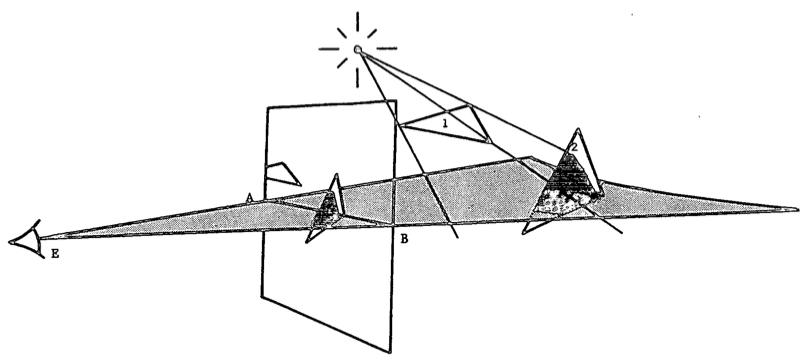
\includegraphics[width=0.9\linewidth]{fig1}
\caption[fig1]{在Appel的算法中,ABE定义了一个“切平面”。多边形1的边投射到多边形2,形成阴影边界,之后投射到图片平面。}
\label{fig:fig1}
\end{figure*}
扫描段的集合由可见线段和切平面的交集决定。
然后对应于光源的量化不可见性(之前已对所有可见顶点算出)会被用来确定那些在阴影中的区段。
更多细节在Appel发表的论文\cite{1}\cite{2}\cite{3}中可见。\\
Bouknight和Kelley开发了一套相似的阴影探测方法\cite{4}\cite{5}。
但是,他们享有一个优势,那就是他们的隐藏表面算法已经基于扫描过程。
通过投射边到正在扫描的表面上,计算出阴影边界,第二次扫描则用来检测这个边界。
主扫描采用图片空间的光栅模式,然后产生第二次扫描,和在物体空间内穿过可见表面的对应路径。
所以,在其他投射到第二次扫描区段的多边形边的地方,就会出现阴影边。\\
一种用来发现所有的可以投射阴影到某个多边形的多边形的步骤被用来减少边投影的计算量。
这个程序将所有的多边形转换成一个伪球形座标空间,而原点在光源处。
多边形之后会测试是否重叠,然后每个多边形都会有一个链接表,使其他可能投射阴影到它上面的多边形可以轻易找到(在图1中,多边形2会链接到多边形1)。
重叠测试的扩展版会引出第二类算法,这将在之后看到。\\
由Bouknight-Kelley提出的典型的通用方法可以解析成两个基本操作:
(1)多边形的阴影优先级顺序 和
(2)计算投射阴影的边界。
值得注意的是,这两个操作相对于显示的隐藏表面算法是独立的,且可以应用到事实上任何基于多边形的算法。\\
可以开发很多基于Bouknight和Kelley的算法的变体。
例如,他们的伪球面重叠测试的算法复杂度是多边形数量的平方。
所以,将可视的物体空间划分成以光源为中心的放射状区域是有利的。
这样就可以将同一个区域内的所有多边形按照阴影优先级顺序排序,而不用参考其他的区域。
确定阴影优先级要求一个特殊的排序方法,例如Newell等人用的方法\cite{9}。
这个算法的行为(同样遵守N方的增长律)在Sutherland等人的论文中有讨论\cite{12}。\\
在有利条件下,分区可以把Bouknight-Kelley(或Newell等人)的N方增长律降低到线性增长律。
分区的增长正比于$ S * (\frac{N}{S})^{2} $,其中S是分区的数量,N是多边形的数量(只要多边形在空间中大体分布保持类似)。
如果增加分区的数量,同时同比例地增加多边形的数量,$ \frac{N}{S} $ 保持不变,那么优先级的步骤就遵守线性增长律。
但是,这个增长速率在受到限制时会变得复杂。当分区足够小时,很大一部分的多边形和分区的边界重叠了,导致多边形的有效数量增加了。
这是因为如果一个多边形横跨了两个分区,那么它必须被两个分区都考虑。
但是,潜在的线性增长速率还是让它成为一个吸引人的方法,不管在这里,还是在通用的分区算法的设计里。\\
第二个基本操作,计算阴影边界,要求一个和裁剪类似的步骤。
正在考虑的多边形必须作为一个窗口,而更高优先级的多边形基于这个窗口进行裁剪。
这个操作的增长速率正比于有阴影多边形的边数和更高优先级多边形的边数的乘积,也是一个N方的增长速率。
但是,分区仍然可以提供一个在有利条件下,总体上线性增长的速率。
(应该注意到,Bouknight和Kelley提出的,在这里使用的链接表在某种程度上是一种优化了的分区。)
有两个因素可以显著减小增长律中的比例常数:
(1)阴影计算只需针对那些可见的多边形进行 和
(2)当一个多边形是完全被阴影遮盖的话,计算可以终止。\\
总结这个部分,应该重新强调的是,在所有阴影算法中,通过仅考虑阴影物体的外围,而不是它的单独的每个多边形,可以减少大量的计算。
这就限制了只要搜索那些产生了可见阴影边界的边。